% Figure 1 — Patient selection flowchart (Cancer Imaging 관례: 세로 주 흐름 + 오른쪽 제외 상자).
% 수치 출처(하드코딩 전 재계산 확인, 2026-09-30):
%   321 / 64 / 257            src/sclc/cohort.py::build_manifest()  (has_image, exclusion_reason)
%   9 / 8 / 2 -> 238          no_report / EVIDENCE_CONFIRMED_LEAK_IDS / report_date 결측(57, 280)
%   LS 72, ES 166, 사건 수      load_trimodal_cohort()  (stage, os_event, pfs_event)
%   진단일 2014-01 ~ 2025-01   data/20260619 SCLC PET 전달용.xlsx '진단일' (238명 기준)
%   fold 크기                   data/splits/trimodal_common_5fold_seed42_v1.csv
% 데이터나 split 이 바뀌면 위 함수로 다시 세고 이 파일의 숫자를 고칠 것.
\documentclass[tikz,border=6pt]{standalone}
% 논문 그림 공통 스타일 (fig1/fig2 가 \input 한다).
% 시각 언어는 Mixture-of-Recursions(MoR) 논문 Fig.1/2 를 따른다:
%   파스텔 채움 + 진남색 얇은 윤곽 + 둥근 모서리, 산세리프 라벨.
% 색 의미(두 그림에서 동일):
%   boxblue   = 영상 모달리티      boxpurple = 임상 모달리티     boxpink = 판독지 모달리티
%   boxgray   = 일반 연산 블록     boxyellow = Cox 관련(head/combiner)
%   dashed    = 동결(frozen) 사전학습 모듈
\usepackage[T1]{fontenc}
\usepackage{helvet}
\renewcommand{\familydefault}{\sfdefault}
\usepackage{amsmath,amssymb}
\usetikzlibrary{positioning,arrows.meta,calc,fit,backgrounds}

\definecolor{navy}{HTML}{2F3B52}
\definecolor{ink}{HTML}{1A1A1A}
\definecolor{ink2}{HTML}{5A5E66}
\definecolor{boxblue}{HTML}{CFE0F7}
\definecolor{boxpink}{HTML}{F6CDD0}
\definecolor{boxpurple}{HTML}{DCD6F3}
\definecolor{boxyellow}{HTML}{FDEEB8}
\definecolor{boxgray}{HTML}{E9E9E9}
\definecolor{cellhold}{HTML}{3F5A8A}
\definecolor{cellfit}{HTML}{F8DD8A}
\definecolor{celleval}{HTML}{F2A4A8}

\tikzset{
  every node/.style={text=ink},
  blk/.style={draw=navy, line width=0.7pt, rounded corners=2.5pt, fill=#1,
              inner xsep=4pt, inner ysep=3pt, font=\footnotesize, align=center},
  blk/.default=boxgray,
  lay/.style={blk=#1, minimum width=30mm, minimum height=6mm},
  inp/.style={blk=#1, minimum width=15mm, minimum height=7mm},
  frozen/.style={lay=boxgray, dashed},
  container/.style={draw=navy, line width=0.8pt, rounded corners=6pt, fill=white, inner sep=6pt},
  armbox/.style={draw=navy, line width=0.6pt, dashed, rounded corners=5pt, inner sep=4pt},
  arr/.style={-{Latex[length=2.2mm,width=1.7mm]}, draw=navy, line width=0.75pt},
  lab/.style={font=\scriptsize, text=ink2, align=center, inner sep=1pt},
  op/.style={circle, draw=navy, line width=0.7pt, fill=white, inner sep=0pt,
             minimum size=4.2mm, font=\scriptsize},
  risk/.style={font=\footnotesize, inner sep=2pt},
  stage/.style={font=\scriptsize\itshape, text=ink2, inner sep=1pt},
  ptitle/.style={font=\footnotesize, align=center, inner sep=2pt},
}

% ---------------------------------------------------------------------------
% 입력 모달리티 아이콘 (fig2 입력단). 글자 라벨 대신 실제 PET-CT MIP 한 장 +
% 임상 표 / 판독지 문서 픽토그램을 쓴다. 모두 약 10.5mm x 12mm 로 크기를 맞추고
% 채움색은 모달리티 색(boxblue/boxpurple/boxpink), 윤곽은 navy 로 본문 도형과 통일.
%   사용: \iconimage{노드이름}{(x,y)}  등. 노드이름으로 화살표를 걸 수 있다.
\newcommand{\iconimage}[2]{%
  \node[blk=boxblue, inner sep=1.1pt, minimum width=0pt, minimum height=0pt] (#1) at #2
       {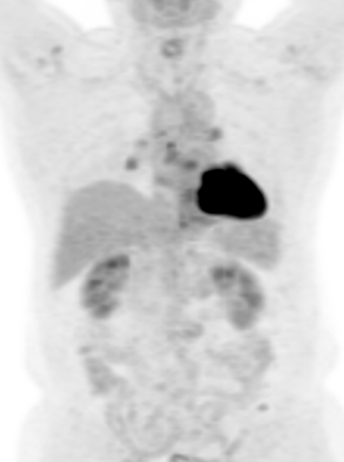
\includegraphics[height=11.8mm]{assets/pet_mip_icon.png}};%
}
\newcommand{\iconclinical}[2]{%
  \begin{scope}[shift={#2}]
    \begin{scope}
      \clip[rounded corners=2.5pt] (-5.25mm,-6mm) rectangle (5.25mm,6mm);
      \fill[boxpurple] (-5.25mm,-6mm) rectangle (5.25mm,6mm);
      \fill[navy!28]   (-5.25mm,3.3mm) rectangle (5.25mm,6mm);
      \draw[navy!45, line width=0.35pt]
        (-5.25mm,3.3mm) -- (5.25mm,3.3mm)  (-5.25mm,0.8mm) -- (5.25mm,0.8mm)
        (-5.25mm,-1.7mm) -- (5.25mm,-1.7mm) (-5.25mm,-4.2mm) -- (5.25mm,-4.2mm)
        (-1.75mm,-6mm) -- (-1.75mm,6mm)     (1.75mm,-6mm) -- (1.75mm,6mm);
    \end{scope}
    \draw[navy, line width=0.7pt, rounded corners=2.5pt] (-5.25mm,-6mm) rectangle (5.25mm,6mm);
    \node[minimum width=10.5mm, minimum height=12mm, inner sep=0pt] (#1) at (0,0) {};
  \end{scope}%
}
\newcommand{\iconreport}[2]{%
  \begin{scope}[shift={#2}]
    \fill[boxpink] (-4.6mm,-6mm) -- (-4.6mm,6mm) -- (1.7mm,6mm) -- (4.6mm,3.1mm) -- (4.6mm,-6mm) -- cycle;
    \draw[navy, line width=0.7pt, rounded corners=1pt]
      (-4.6mm,-6mm) -- (-4.6mm,6mm) -- (1.7mm,6mm) -- (4.6mm,3.1mm) -- (4.6mm,-6mm) -- cycle;
    \fill[navy!20] (1.7mm,6mm) -- (1.7mm,3.1mm) -- (4.6mm,3.1mm) -- cycle;
    \draw[navy, line width=0.55pt] (1.7mm,6mm) -- (1.7mm,3.1mm) -- (4.6mm,3.1mm);
    \draw[navy!55, line width=0.5pt]
      (-2.9mm,1.4mm) -- (2.9mm,1.4mm)  (-2.9mm,-0.4mm) -- (2.9mm,-0.4mm)
      (-2.9mm,-2.2mm) -- (2.9mm,-2.2mm) (-2.9mm,-4.0mm) -- (0.9mm,-4.0mm);
    \node[minimum width=9.2mm, minimum height=12mm, inner sep=0pt] (#1) at (0,0) {};
  \end{scope}%
}

\begin{document}
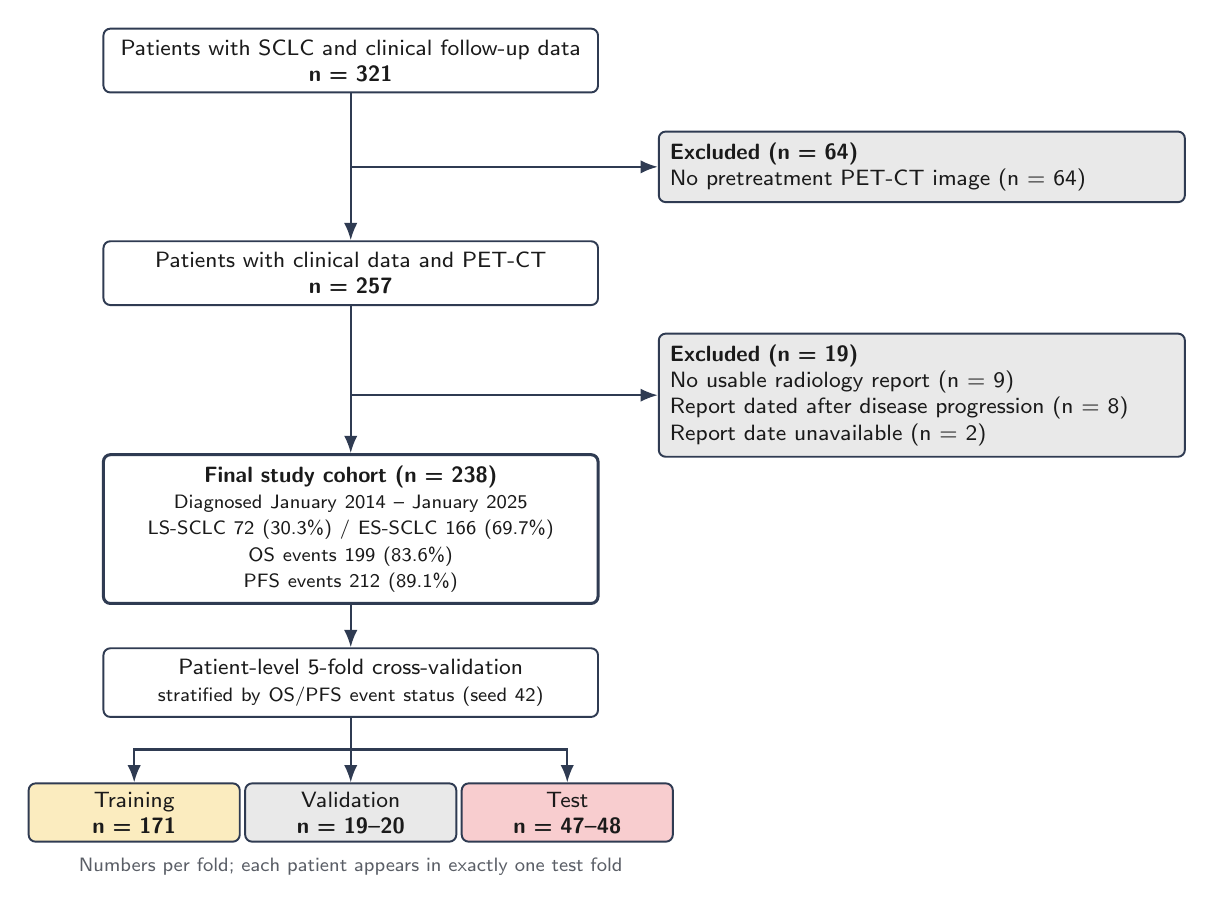
\begin{tikzpicture}[x=1cm,y=1cm,
  flow/.style={blk=white, text width=60mm, inner ysep=4pt},
  excl/.style={blk=boxgray, text width=64mm, align=left, anchor=west, inner ysep=4pt},
  part/.style={blk=#1, text width=24mm, inner ysep=3pt},
  line/.style={draw=navy, line width=0.75pt},
]

% ---------------- main flow ----------------
\node[flow] (all) at (0,0)
  {Patients with SCLC and clinical follow-up data\\
   \textbf{n = 321}};

\coordinate (j1) at (0,-1.35);
\node[excl] (ex1) at (3.9,-1.35)
  {\textbf{Excluded (n = 64)}\\
   No pretreatment PET-CT image (n = 64)};

\node[flow] (img) at (0,-2.7)
  {Patients with clinical data and PET-CT\\
   \textbf{n = 257}};

\coordinate (j2) at (0,-4.25);
\node[excl] (ex2) at (3.9,-4.25)
  {\textbf{Excluded (n = 19)}\\
   No usable radiology report (n = 9)\\
   Report dated after disease progression (n = 8)\\
   Report date unavailable (n = 2)};

\node[flow, line width=1.1pt] (final) at (0,-5.95)
  {\textbf{Final study cohort (n = 238)}\\
   {\scriptsize Diagnosed January 2014 -- January 2025}\\
   {\scriptsize LS-SCLC 72 (30.3\%) / ES-SCLC 166 (69.7\%)}\\
   {\scriptsize OS events 199 (83.6\%)}\\
   {\scriptsize PFS events 212 (89.1\%)}};

\node[flow] (cv) at (0,-7.9)
  {Patient-level 5-fold cross-validation\\
   {\scriptsize stratified by OS/PFS event status (seed 42)}};

% per-fold partitions (색은 fig1 late-fusion 격자와 같음: fit=노랑, eval=분홍)
\node[part=cellfit!55]  (tr) at (-2.75,-9.55) {Training\\ \textbf{n = 171}};
\node[part=boxgray]     (va) at (0,-9.55)     {Validation\\ \textbf{n = 19--20}};
\node[part=celleval!55] (te) at (2.75,-9.55)  {Test\\ \textbf{n = 47--48}};
\node[lab, below=1.5mm of va]
  {Numbers per fold; each patient appears in exactly one test fold};

% ---------------- arrows ----------------
\draw[arr] (all) -- (img);
\draw[arr] (img) -- (final);
\draw[arr] (final) -- (cv);
\draw[arr] (j1) -- (ex1.west);
\draw[arr] (j2) -- (ex2.west);

\coordinate (fork) at (0,-8.75);
\draw[line] (cv.south) -- (fork);
\draw[arr] (fork) -| (tr.north);
\draw[arr] (fork) -- (va.north);
\draw[arr] (fork) -| (te.north);

\end{tikzpicture}
\end{document}
